\chapter{Manual de usuario}
\section{Instalación}
O plugin pode instalarse desde a opción 'Administrar e instalar plugins' no menú Plugins do QGIS.
\begin{figure}[hbtp]
\centering
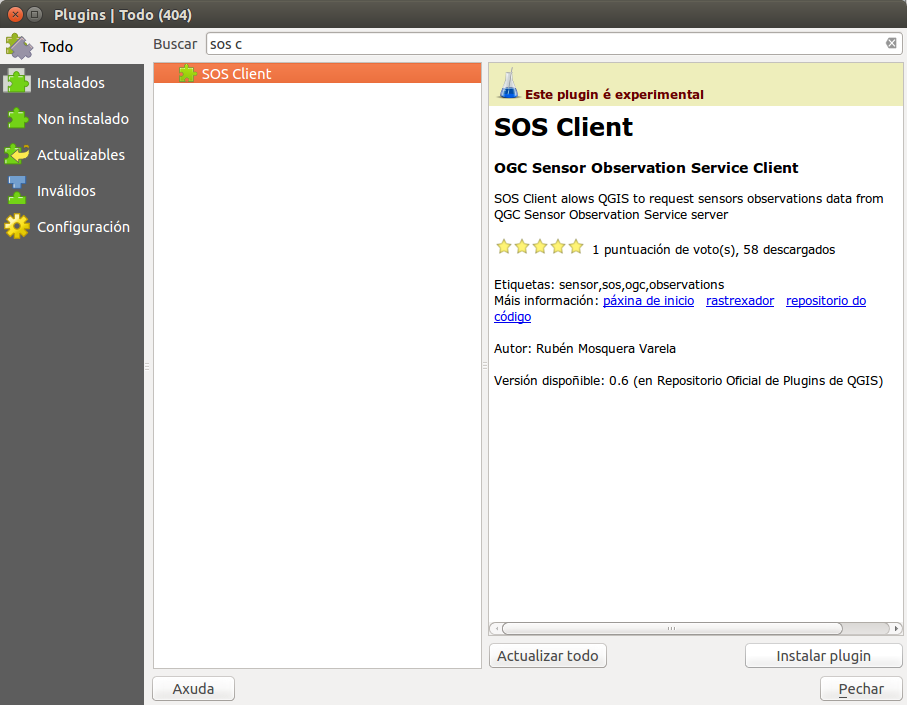
\includegraphics[width=0.8\textwidth]{images/manual/instalar.png}
\caption{Pantalla de instalación do plugin}
\label{fig:install}
\end{figure}

Unha vez instalado engadirase unha nova entrada no menú Web e tres novas accións na barra de ferramentas:
\begin{figure}[hbtp]
\centering
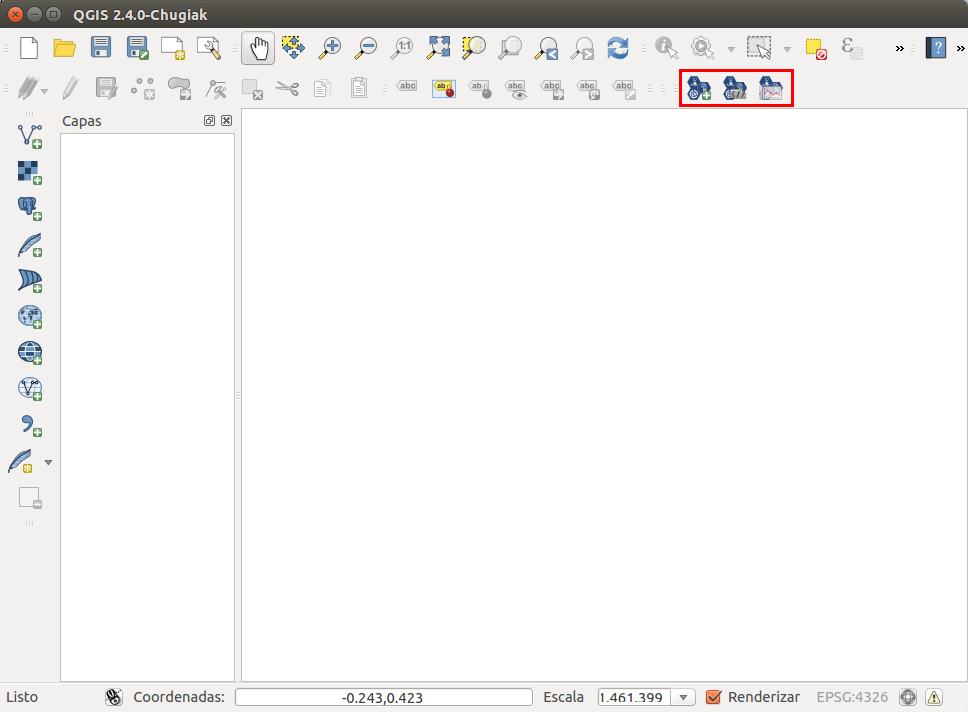
\includegraphics[width=0.8\textwidth]{images/manual/toolbar.png}
\caption{Barra de ferramentas do plugin}
\label{fig:toolbar}
\end{figure}

\begin{description}
\item [{
\includegraphics[width=24px]{images/manual/icon_add.png}}] Mostra o diálogo para conectar con un servidor SOS e engadir unha capa de observacións. 
\item [{
\includegraphics[width=24px]{images/manual/icon_xml.png}}] Visualiza o ficheiro XML usado para xerar a capa activa. 
\item [{
\includegraphics[width=24px]{images/manual/icon_plot.png}}] Xera unha gráfica coas observacións correspondentes ás entidades seleccionadas na capa activa.
\end{description}

\section{Crear capa de observacións}
Ó pulsar a acción 
\includegraphics[width=16px]{images/manual/icon_add.png} mostrarase o formulario da figura TODO. Neste formulario pódese xestionar a lista de servidores cos botóns Novo, Editar e Eliminar, e co botón Conectar visualizar as capacidades do servidor seleccionado.
\begin{figure}[hbtp]
\centering
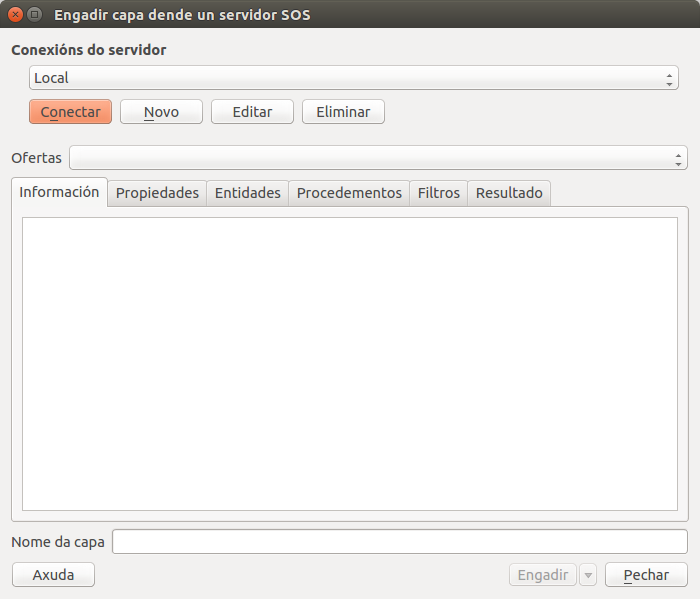
\includegraphics[width=\textwidth]{images/manual/tabInfo-limpia.png}
\caption{Diálogo de conexión co servidor, sen datos}
\label{fig:tabInfo-limpia}
\end{figure}

Unha vez se conectou con un servidor móstranse as súas capacidades na lapela Información (figura \ref{fig:tabInfo}).
\begin{figure}[hbtp]
\centering
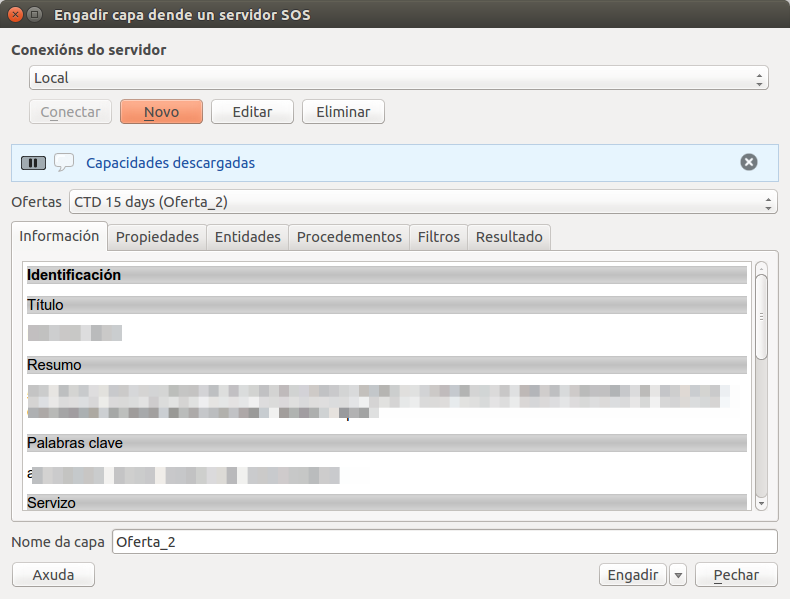
\includegraphics[width=\textwidth]{images/manual/tabInfo.png}
\caption{Diálogo de conexión co servidor, con datos}
\label{fig:tabInfo}
\end{figure}

Para obter as observacións débese seleccionar unha oferta no campo Ofertas e pódese modificar no Nome da capa. As distintas lapelas do formulario descríbense no cadro \ref{tab:lapelas}:
\begin{table}	
\begin{tabularx}{\textwidth}{cX}
	\raisebox{-0.8\totalheight}{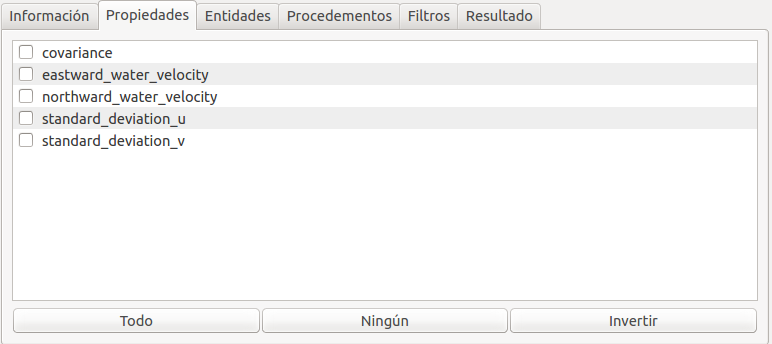
\includegraphics[width=0.4\textwidth]{images/manual/tabPropiedades.png}} & 
	Lista de propiedades da oferta. Pode seleccionar unha ou varias.\\
	\\
	\raisebox{-0.8\totalheight}{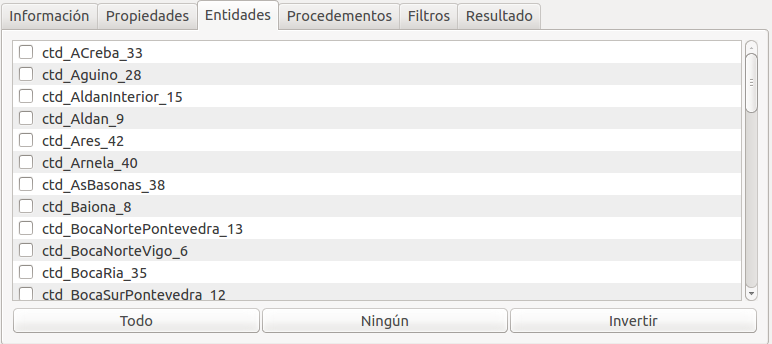
\includegraphics[width=0.4\textwidth]{images/manual/tabEntidades.png}} & Lista de entidades da oferta. Pode seleccionar varias ou ningunha.\\
	\\
	\raisebox{-0.8\totalheight}{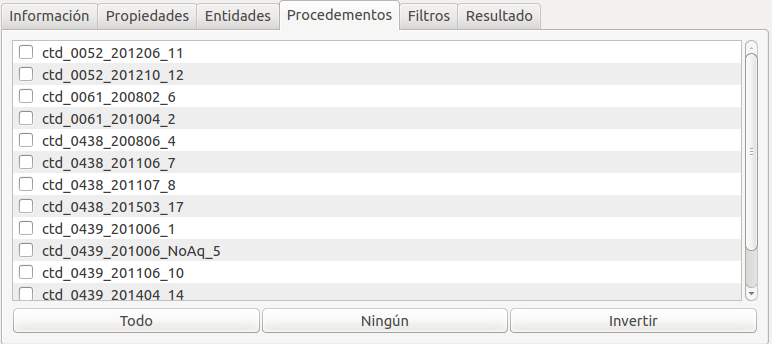
\includegraphics[width=0.4\textwidth]{images/manual/tabProcedementos.png}} & Lista de procedementos. Pode seleccionar varios ou ningún.\\
	\\
	\raisebox{-0.8\totalheight}{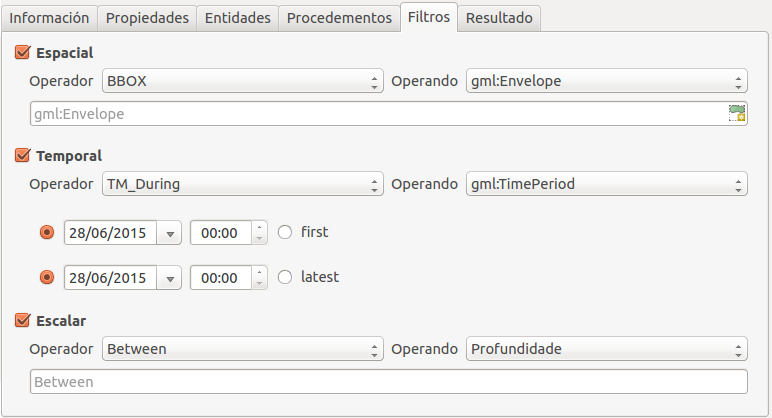
\includegraphics[width=0.4\textwidth]{images/manual/tabFiltros.png}} & Filtros dispoñibles. Pódense activar varios ó mesmo tempo. No caso do espacial, pulsando na icona poderase seleccionar a xeometría a consultar debuxando no mapa como se amosa na figura \ref{fig:spatialtool}.\\
	\\
	\raisebox{-0.8\totalheight}{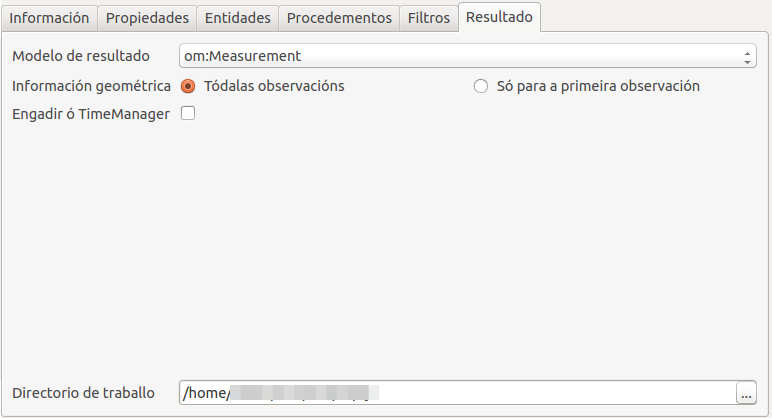
\includegraphics[width=0.4\textwidth]{images/manual/tabResultado.png}} & Pódese seleccionar o modelo de resultado entre os dispoñibles para o servidor. Permite indicar se todas as entidades terán información xeométrica ou so a primeira para cada \emph{foi} e seleccionar se engadir a capa ó TimeManager. Tamén se pode seleccionar o directorio de traballo no que se gardan os datos descargados.\\
\end{tabularx}
\caption{Lapelas do formulario de consulta ó SOS}
\label{tab:lapelas}
\end{table}

\begin{figure}[hbtp]
\centering
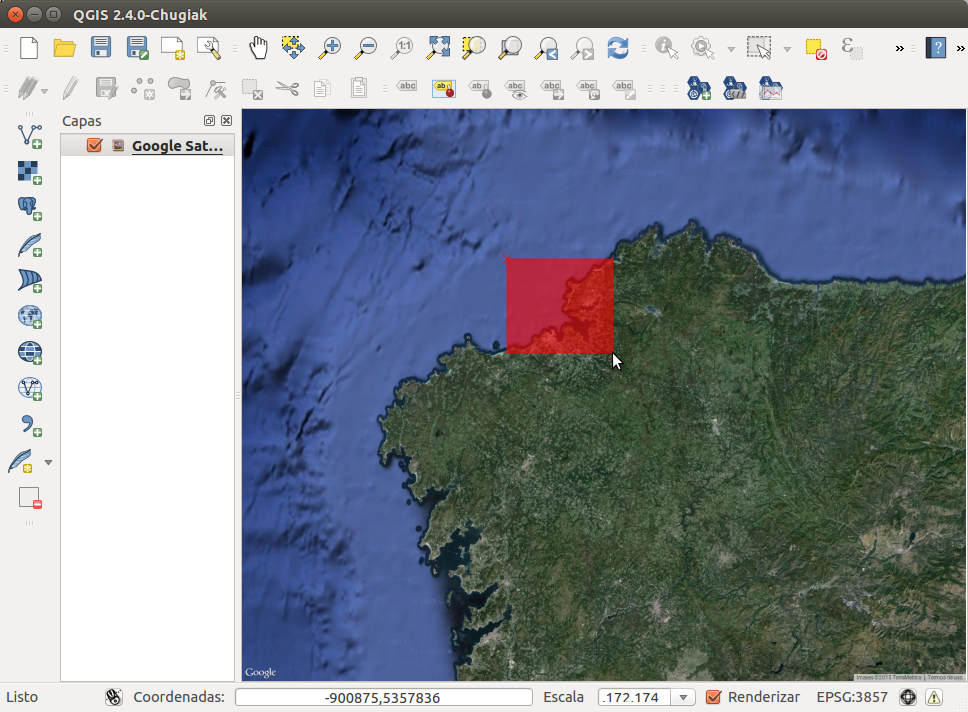
\includegraphics[width=\textwidth]{images/manual/spatialtool.png}
\caption{Ferramenta de selección espacial}
\label{fig:spatialtool}
\end{figure}

Unha vez seleccionadas as opcións desexadas pódese engadir a capa ó QGIS pulsando no botón Engadir, ou cambiar o XML a enviar antes de engadir a capa co botón 'Editar petición', como se ve na figura \ref{fig:editarPeticion}.

\begin{figure}[hbtp]
\centering
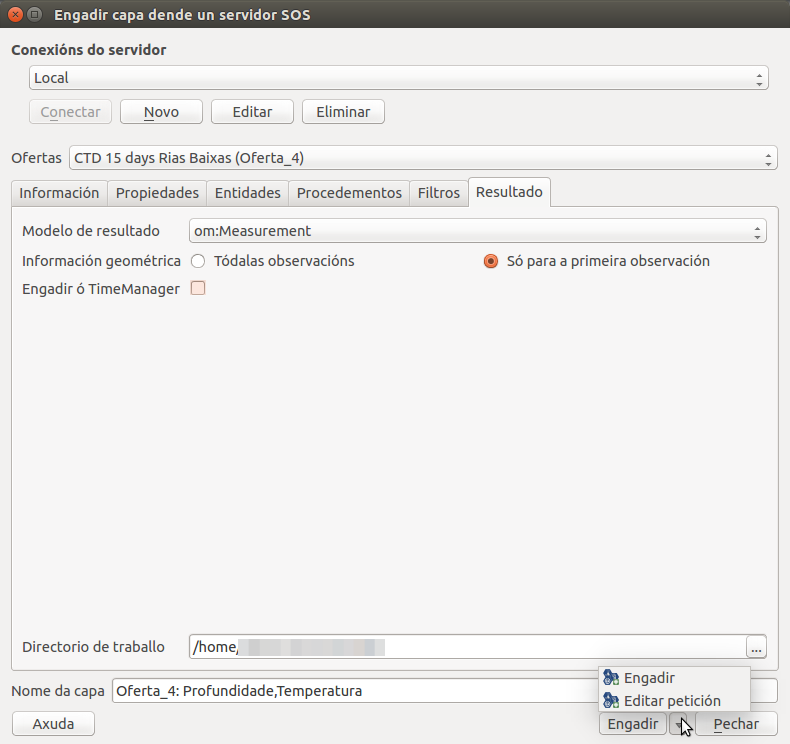
\includegraphics[width=\textwidth]{images/manual/editar_peticion.png}
\caption{Engadir capa SOS}
\label{fig:editarPeticion}
\end{figure}

\section{Gráficos en dúas dimensións}

Para visualizar un gráfico é necesario que a capa activa teña unha ou máis entidades seleccionadas, e despois premer no botón 
\includegraphics[width=16px]{images/manual/icon_plot.png}, como se amosa na figura \ref{fig:ejecutarSOSPlot}.

\begin{figure}[hbtp]
\centering
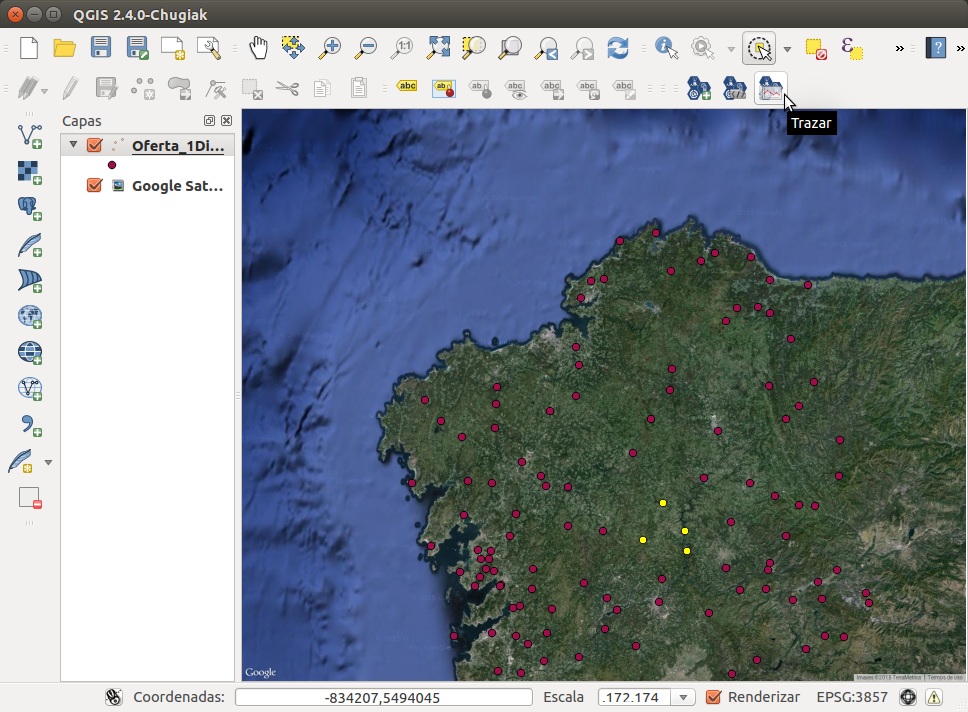
\includegraphics[width=\textwidth]{images/manual/ejecutar_sosplot.png}
\caption{Executar ferramenta SOS Plot}
\label{fig:ejecutarSOSPlot}
\end{figure}

Esta operación abrirá unha nova ventá (figura \ref{fig:sosplot}) na que se visualizará a gráfica, e na que se poden editar as opcións do mesmo e interactuar coa gráfica.

\begin{figure}[hbtp]
\centering
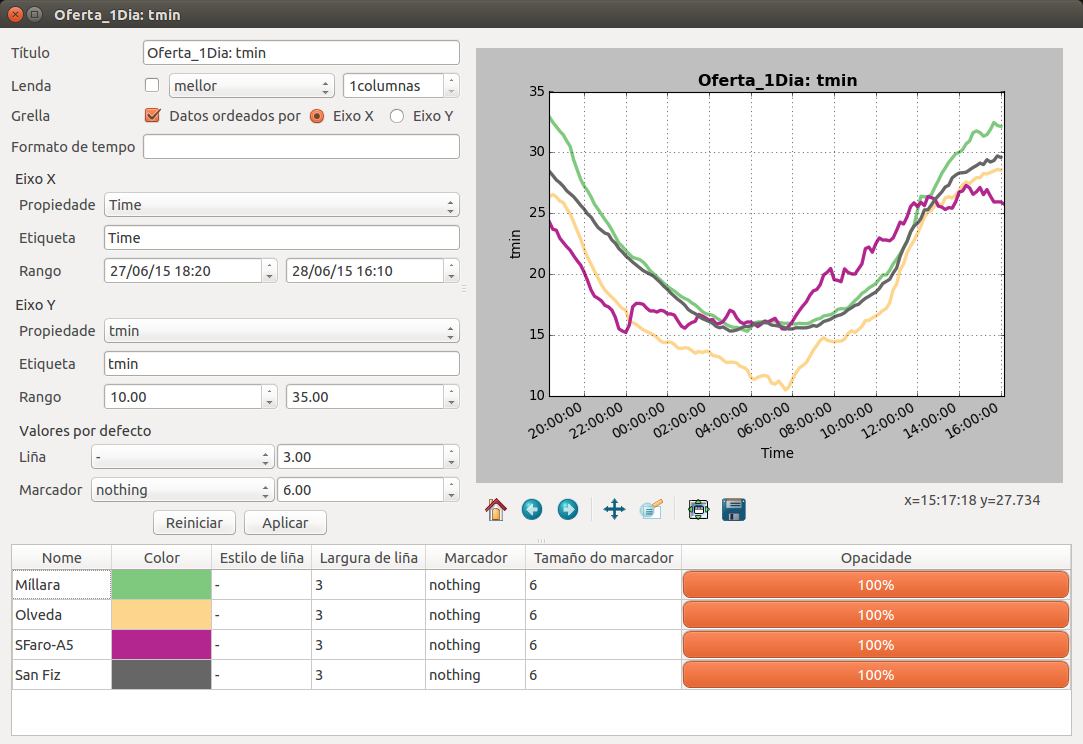
\includegraphics[width=\textwidth]{images/manual/sosplot.png}
\caption{SOS Plot: Gráfica de varias series}
\label{fig:sosplot}
\end{figure}

Neste formulario pódese editar o título do gráfico e dos eixos, a propiedade a representar en cada eixo e os límites dos mesmos, o formato no que representar o tempo, a inclusión dunha lenda, e o estilo e cor de liña e marcador de cada unha das series debuxadas. Amais sobre a gráfica pódese facer zoom, desprazala e gardar a imaxe.